\documentclass[11pt]{article}

\usepackage[letterpaper,top=2cm,bottom=2cm,left=2.5cm,right=2.5cm,marginparwidth=1.75cm]{geometry}

%packages
\usepackage{amsmath}
\usepackage{graphicx}
\usepackage{amssymb}
\usepackage{algorithm}
\usepackage{algpseudocode}
\usepackage{color,soul}
\usepackage{mathtools}
% \usepackage{subfig}
\usepackage{subcaption}
\usepackage{caption}

% Edits by John:
% Use hyperref when you're referencing anything - in particular, use the \autoref{} command - it's great. One exception: anything in mathmode should be referenced using \eqref{} instead; \autoref{} calls all mathmode objects "equations", even when they're not equations (definitions, inequalities, propositions, statements, etc.), so it's better to use the \eqref{} function.
\usepackage[colorlinks, linkcolor=blue, citecolor=blue, urlcolor=blue]{hyperref}
% Use the align (or similar) environment, rather than built-in latex commands for math statements. That way, things can be aligned properly and equations will be numbered and referencable. The equation below assigns equation numbers based upon the current section.

\numberwithin{equation}{section}
% Use the amsthm environents to define theorems, remarks, definitions, etc., with commands of the form \begin{definition}[DEFINITION ITTLE]
\usepackage{amsthm}% provides the environments
\theoremstyle{definition}% provides a style for definitions - this affects all downstream \newtheorem statements until \theoremstyle is used again.
\newtheorem{theorem}{Theorem}
\newtheorem{definition}{Definition}[section]% numbers definitions within sections
% The singular of "matrices" is "matrix", not "matrice" - the abnormal singular-plural pair is an importation from Latin.
% Use \url{} for hyperlinks (I changed the pytorch link). I think this is included in hyperref, but it may be in base LaTeX.

\DeclarePairedDelimiter\ceil{\lceil}{\rceil}
\DeclarePairedDelimiter\floor{\lfloor}{\rfloor}
\newcommand{\pluseq}{\mathrel{+}=}
\newcommand{\asteq}{\mathrel{*}=}

\usepackage[dvipsnames]{xcolor}

\definecolor{lavender}{RGB}{214, 111, 208}
\colorlet{lavender}{lavender!50}

\newcommand{\hlinfo}[1]{{\sethlcolor{lavender}\hl{#1}}}
\newcommand{\note}[1]{\textcolor{red}{[#1]}}

\usepackage{tikz}

\setlength\parindent{0pt}

\begin{document}

\noindent
\begin{center}
    \section*{\centering{Week 2 Notes}}
    \subsection*{\centering{\emph{Lectures 3 \& 4}}}
    \emph{University of Massachusetts Amherst}, CS389
\end{center}

\section{Neural Networks (lecture 3)}

\begin{definition}[Multi-dimensional data] A \emph{multi-dimensional data} that has $n$ number of data with $d$ number of features can be written as\footnote{Note that this array is transposed because $X$ is a row vector and each $X^{(i)}$ is a d-dimensional column vector}:
    \begin{align}
        X = \left [ X^{(1)}, X^{(2)}, ..., X^{(n)} \right ]^{T}
    \end{align}
where $X^{(i)}$ is the $i^{\text{th}}$ data\footnote{The reason why we use the $X^{(i)}$ notation is because $X^{(i)}$ is a vector and sometimes we need to refer to the elements of that vector \cite{MIT}}. A single data, $X^{(i)}$ is a d-dimensional vector which has $d$ number of features. For example, the features for a weather data may include humidity, temperature, air speed, etc. Every data is represented as a row and each feature as a column. Formally we write a single data as:
    \begin{align}
        X^{(i)} = \left [ X_{1}^{(i)}, X_{2}^{(i)}, ..., X_{d}^{(i)} \right ]
    \end{align}
Putting all this together, our multi dimensional data is a matrix with dimensions $(n \times d)$:
    \begin{align}
        X = \begin{bmatrix}
            X_{1}^{(1)} & \cdots & X_{d}^{(1)} \\
            \vdots & \ddots & \vdots \\
            X_{1}^{(n)} & \cdots & X_{d}^{(n)} 
        \end{bmatrix}
    \end{align}


\end{definition}

\subsection{Perceptron}
\begin{definition}[Perceptron]
    A \emph{perceptron} is a computational model of a biological neuron. A graphical visualization of a perceptron can be seen in \autoref{fig:perceptron},
\end{definition}

\begin{figure}[h]
    \begin{center}
        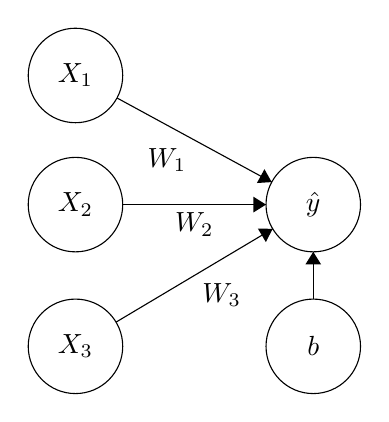
\begin{tikzpicture}[scale=0.2]
        \tikzstyle{every node}+=[inner sep=0pt]
        \draw [black] (21.5,-13.7) circle (3);
        \draw (21.5,-13.7) node {$X_1$};
        \draw [black] (21.5,-21.9) circle (3);
        \draw (21.5,-21.9) node {$X_2$};
        \draw [black] (21.5,-30.9) circle (3);
        \draw (21.5,-30.9) node {$X_3$};
        \draw [black] (36.6,-21.9) circle (3);
        \draw (36.6,-21.9) node {$\hat{y}$};
        \draw [black] (36.6,-30.9) circle (3);
        \draw (36.6,-30.9) node {$b$};
        \draw [black] (36.6,-27.9) -- (36.6,-24.9);
        \fill [black] (36.6,-24.9) -- (36.1,-25.7) -- (37.1,-25.7);
        \draw [black] (24.5,-21.9) -- (33.6,-21.9);
        \fill [black] (33.6,-21.9) -- (32.8,-21.4) -- (32.8,-22.4);
        \draw (29.05,-22.4) node [below] {$W_2$};
        \draw [black] (24.08,-29.36) -- (34.02,-23.44);
        \fill [black] (34.02,-23.44) -- (33.08,-23.42) -- (33.59,-24.28);
        \draw (30.79,-26.9) node [below] {$W_3$};
        \draw [black] (24.14,-15.13) -- (33.96,-20.47);
        \fill [black] (33.96,-20.47) -- (33.5,-19.65) -- (33.02,-20.53);
        \draw (27.31,-18.3) node [below] {$W_1$};
        \end{tikzpicture}
    \end{center}
    \caption{A single-layer perceptron}
    \label{fig:perceptron}
\end{figure}

where the vertices $X_i$ are the input features, the edges $W_i$ are the weighted connections, the vertex $b$ is the bias term, and the vertex $Y'$ is the output. We can write this mathematically as:
\begin{align}
    \hat{y} = \phi(W^{T}X + b)
\end{align}

where $\phi$ is a non-linearity function, also known as an activation function (topic of next week). 

\subsection{Classification}

In a classification problem, we want to learn to predict discrete classes which the input belongs to. 

\begin{definition}[Binary classification] Is a supervised learning algorithm that \emph{categorizes the data into one of two classes}.
\end{definition}

Recall that a linear model is defined as: 
\begin{align}
    \hat{y} = \phi \left (\sum_{j=1}^{m}{w_j \cdot X_j + b} \right ) = \phi (W^{T}X + b)
\end{align}
% 
where the output $\hat{y} \in \mathbb{R}$ and we can apply a type of boolean function (i.e. the \emph{sign} activation function) so that the output $\hat{y} \in \{-1, +1\}$. Given a fixed model, the binary classifier is defined as:
\begin{align}
    \hat{y} = \text{sign}(W^{T}X + b) = \begin{cases}
        +1 & \text{if $W^{T}X + b > 0$}\\
        -1 & \text{otherwise}
    \end{cases}
\end{align}
As can be seen in \autoref{fig:linear_classifier}, the points that are on the same side as the normal vector to the hyperplane is the positive half-spaces are classified as positive. Likewise, the other half-space is negative and all points are classified as negative \cite{MIT}. 
\begin{figure}[h]%
    \centering
    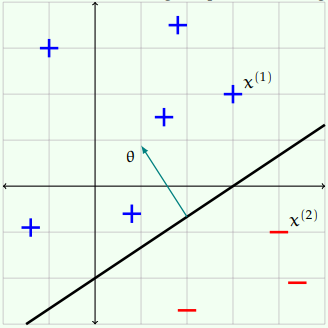
\includegraphics[width=8cm]{./Figs/linear_classifer.png}%
    \qquad
    \caption{Binary Classification Example. The $\theta$ is the same variable as $W$ \cite{MIT}}%
    \label{fig:linear_classifier}%
\end{figure}


% activation function is sign function

\subsection{Linear Separability}

% Previously we said we can do bclass if w > 0 etc...

\begin{theorem}
    \emph{If the dataset, $D$, is linearly separable, then the perceptron algorithm is guaranteed to find a linear separator} \cite{MIT}
\end{theorem}

How would one \emph{formally describe linear separability?} This is beyond the scope for this class, but you can refer to this \href{https://openlearninglibrary.mit.edu/assets/courseware/v1/8f4f9aca5581dde50291b0d0e29d0148/asset-v1:MITx+6.036+1T2019+type@asset+block/notes_chapter_The_Perceptron.pdf}{MIT lecture notes (pg. 4)} for a detailed explanation. The intuition is if the shortest distance of a point to the hyperplane (the norm) is positive for all points then the dataset is classified correctly. You can use \autoref{fig:linear_classifier} to help with this visualization. Understanding this helps us understand why the perceptron is unable to solve XOR.

\subsection{Regression}

\begin{definition}[Regression]
    Predict continuous outputs ($\hat{y} \in \mathbb{R}$) that are close to the true values
\end{definition}

\section{Stochastic Gradient Descent implementation (lecture 4)}

Hopefully, we now have a mathematical understanding and an intuition of all the main components of a supervised machine learning model. We can now start implementing a very simple SGD. Recall that in a SGD, we want to update the parameters $W$ and $b$ after every single training data.

% SGD algorithm
\begin{algorithm}
    \caption{Stochastic Gradient Descent algorithm}
    \begin{algorithmic}[1]
        \For{$e$ in range Epoch} \Comment{number of epochs}
            \For{$X^{(i)}$ in $X$} \Comment{loop through entire dataset}
                \State{$\hat{y}^{(i)} = X^{(i)}W^{T} + b$} \Comment{our model's prediction for input $X^{(i)}$}
                \State{Loss$^{(i)} = \frac{1}{2} \sum{(y^{(i)} - \hat{y}^{(i)})^{2}}$ } \Comment{calculate MSE loss of prediction with actual}
                \State{$W = W - \alpha \frac{\partial L^{(i)}}{\partial W}$}    \Comment{update weight}
                \State{$b = b - \alpha \frac{\partial L^{(i)}}{\partial b}$} \Comment{update bias}
            \EndFor
        \EndFor
    \end{algorithmic}
\end{algorithm}

% Gradient of loss
\subsection{Calculating Gradient of Loss}

The gradient of loss can be written as $\nabla_W \text{Loss}$ or  $\frac{\partial L}{\partial W}$. The gradient of loss is a vector of partial derivatives. We will often use terms such as “the gradient on x” instead of the technically correct phrase “the partial derivative on x” for simplicity \cite{Stanford}: 
\begin{align}
    \nabla_W \text{Loss} = \frac{\partial L}{\partial W} = \left( \frac{\partial L}{\partial w_1}, \frac{\partial L}{\partial w_2}, ..., \frac{\partial L}{\partial w_m} \right)
\end{align}
Using the chain rule we have:
\begin{align}
    \frac{\partial L}{\partial W_j} = \frac{\partial \hat{y}}{\partial W_j} \frac{\partial L}{\partial \hat{y}}
\end{align}
Now recall that $\hat{y} = W^{T}X + b$ and $L = \frac{1}{2} \sum{(y^{(i)} - \hat{y}^{(i)})^{2}}$ , therefore:
\begin{align}
    \frac{\partial \hat{y}}{\partial W_j} = X_j^{(i)}
\end{align}
\begin{align}
    \frac{\partial \hat{L}}{\partial \hat{y}} = \hat{y}^{(i)} - y^{(i)}
\end{align}
\begin{align}
    \nabla_W \text{Loss} = \frac{\partial L}{\partial W} = \left[ X_1^{(i)} \cdot (\hat{y}^{(i)}-y^{(i)}), X_2^{(i)} \cdot (\hat{y}^{(i)}-y^{(i)}), ..., X_n^{(i)} \cdot (\hat{y}^{(i)}-y^{(i)}) \right]
\end{align}
\begin{align}
    \therefore \frac{\partial L}{\partial W} = \left[ X_1^{(i)}, X_2^{(i)}, ..., X_n^{(i)} \right] \cdot (\hat{y}^{(i)}-y^{(i)}) = X^{(i)} \cdot (\hat{y}^{(i)}-y^{(i)})
\end{align}


\begin{thebibliography}{2}
    \bibitem{DrCoop} Cooper.

    \bibitem{MIT} {MIT Open Learning Library, 6.036, Spring 2020, \url{https://openlearninglibrary.mit.edu/assets/courseware/v1/2481f8f2964716032b134db99e369b81/asset-v1:MITx+6.036+1T2019+type@asset+block/notes_chapter_Introduction.pdf}}

    \bibitem{Stanford} Fei-Fei Li, Jiajun Wu, and Ruohan Gao, Stanford CS231n, Spring 2022. \url{https://web.archive.org/web/20230109135558/https://cs231n.github.io/}

\end{thebibliography}

\end{document}
